\documentclass[12pt,]{article}


%\usepackage{baskervillef}%polskie znaki może nie

%flow chatry
\usepackage{tikz}
\usetikzlibrary{shapes.geometric, arrows}
\usepackage{amssymb}
\usepackage{float}

\title{Sprawozadanie lernicng}
\author{Tymon Łazowy}
\date{123,2123,12}


\tikzstyle{startstop} = [ellipse, rounded corners, minimum width=2cm, minimum height=1cm,text centered, draw=black,thick,fill=red!0]

\tikzstyle{io} = [trapezium,
trapezium stretches=true,
trapezium left angle=70,
trapezium right angle=110,
thick,minimum width=2cm,
minimum height=0.85cm,
text centered,
draw=black,
fill=blue!0]

\tikzstyle{process} = [rectangle,
minimum width=3cm,
minimum height=0.85cm,
text centered,
text width=3cm,draw=black,thick,fill=orange!0]

\tikzstyle{decision} = [diamond,minimum width=1cm, minimum height=1cm, text centered, draw=black, fill=green!0,thick]

\tikzstyle{arrow} = [thick,->,>=stealth]

\begin{document}
 D: a,b,c parametry $\in$ \{7; 12; 16\}
 
 S: sr średnia parametrów $\in$ \{11,67\}
\begin{figure}[h]
   
    \caption{1.5 flowchart} 
    \centering  
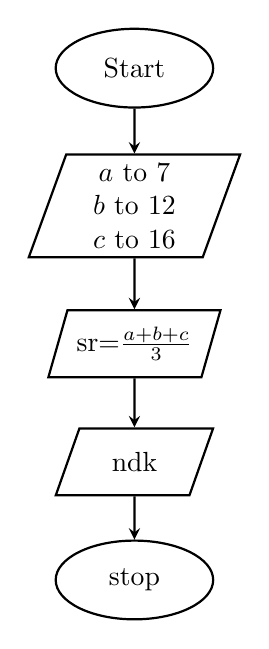
\begin{tikzpicture}[node distance=1.5cm]

\node (start) [startstop] {Start};
\node (out1) [io, below of=start,text width=1.5cm,yshift=-0.25cm] {$a$ to 7

$b$ to 12

$c$ to 16};
\node (in1) [io, below of=out1,yshift=-0.25cm] {sr=$\frac{a+b+c}{3}$};
\node (out2) [io, below of=in1]{ndk};
\node (stop) [startstop, below of =out2]{stop};

\draw [arrow] (start) -- (out1);
\draw [arrow] (out1) -- (in1);
\draw [arrow] (in1) -- (out2);
\draw [arrow] (out2) -- (stop);



\end{tikzpicture}
    
    \label{flow5}
\end{figure}
\end{document}